% !TEX TS-program = xelatex
% !TEX encoding = UTF-8
% !Mode:: "TeX:UTF-8"

\documentclass[onecolumn,oneside]{SUSTechHomework}

\usepackage{float}
\usepackage{multirow}

\author{胡玉斌}
\sid{11712121}
\title{Assignment3}
\coursecode{CS323}
\coursename{Compilers}

\begin{document}
  \maketitle

\section{(Grammar Basics): Consider the following context-free grammar $G$:}

  $$S \rightarrow SS + | SS * | a$$

  \subsection{Is the string $a+a*a$ in $L(G)$? [10points]}

  \paragraph{No. $+$ must have at lease 2 terminal before, but it has only one.}

  \subsection{Give a leftmost derivation for the string $aa *  aa + *.$ [10points]}

  \paragraph{$S \rightarrow SS* \rightarrow SS+S* \rightarrow aS+S* \rightarrow aa*S* \rightarrow aa*SS+* \rightarrow aa*aS+* \rightarrow aa*aa+*$}

  \subsection{Give a rightmost derivation for the string $aa * aa + *.$ [10points]}

  \paragraph{$S \rightarrow SS* \rightarrow SSS+* \rightarrow SSa+* \rightarrow Saa+* \rightarrow SS*aa+* \rightarrow Sa*aa+* \rightarrow aa*aa+*$}

  \subsection{Give a parse tree for the string $aa * aa + *.$ [10points]}

  \begin{figure}[H]
    \centering
    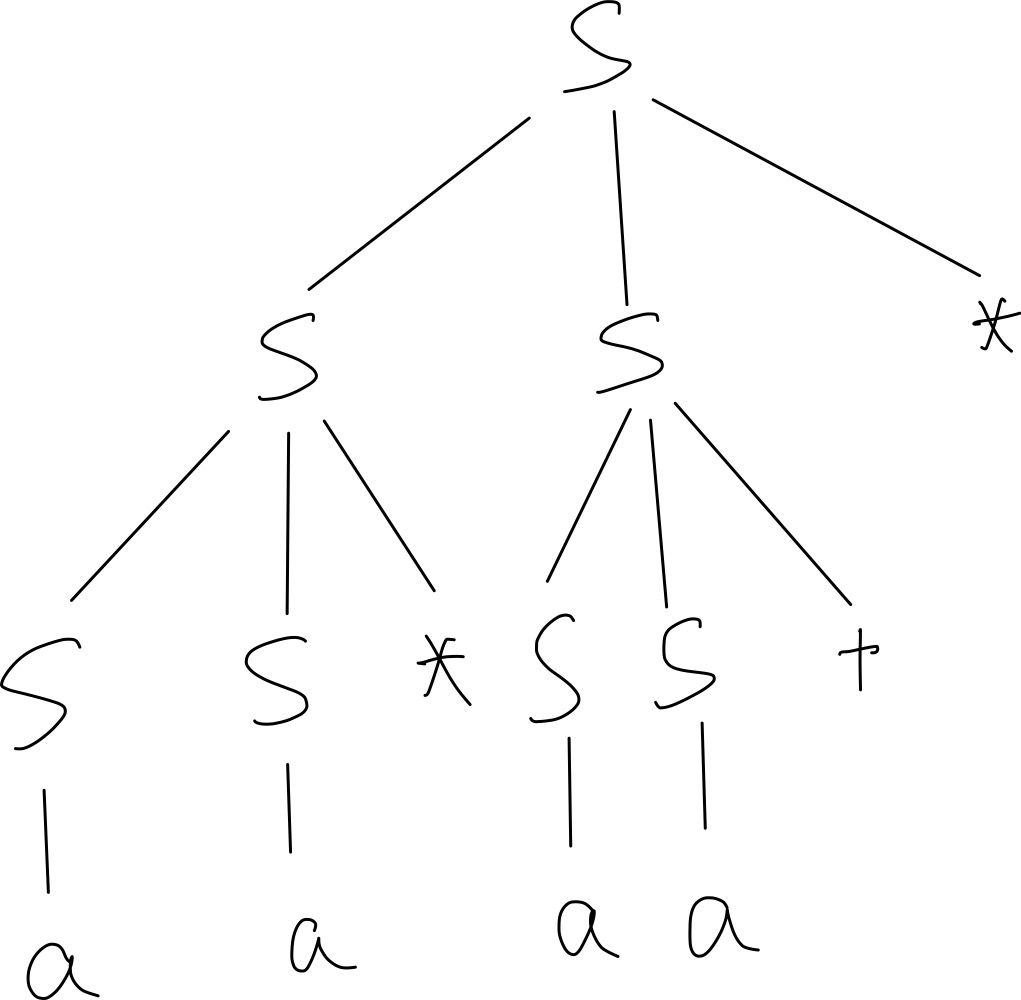
\includegraphics[width=0.30\textwidth]{img/pic1.jpg}
    \caption{paser tree}
  \end{figure}

  \subsection{Give an equivalent grammar without immediate left recursions. [10points]}

  $$S \rightarrow aS'$$
  $$S' \rightarrow S+S' | S*S' | \epsilon$$

\newpage

\section{(Top-Down Parsing): Consider the following grammar $G$:}

  $$S \rightarrow aB$$
  $$B \rightarrow S + B | \epsilon$$

  \subsection{Construct the predictive parsing table for $G$. Please put down the detailed steps, including the calculation of FIRST and FOLLOW sets. [25 points]}

  non-terminal = $\{S, B\}$

  terminal = $\{a, +, \epsilon\}$

  \begin{itemize}
    \item FIRST sets
    \begin{itemize}
      \item FISTR(S) = $\{a\}$ 
      \item FIRST(B) = FIRST(S) $\cup \epsilon$ = $\{a, \epsilon\}$
    \end{itemize}
    \item FOLLOW sets
    \begin{itemize}
      \item FOLLOW(S) = $\{\$, +\}$
      \item FOLLOW(B) = $\{\$, +\}$
    \end{itemize}
  \end{itemize}

  \begin{table}[H]
    \begin{tabular}{|l|l|l|l|l|}
    \hline
      & a                   & +                 & \$                &  \\ \hline
    S & $S \rightarrow aB$  &                   &                   &  \\ \hline
    B & $B \rightarrow S+B$ & $B \rightarrow \epsilon$ & $B \rightarrow \epsilon$ &  \\ \hline
    \end{tabular}
  \end{table}
  
  \subsection{Is the grammar $LL(1)$? [5 points]}

  Recursive-descent parsers needing no backtracking can be constructed for a class of grammars called $LL(1)$. The grammar should hold:
  \begin{itemize}
    \item There is no terminal $\alpha$ such that $\alpha$ and $\beta$ derive strings beginning with $\alpha$
    \item At most one of $\alpha$ and $\beta$ can derive the empty string
    \item If $\beta \Rightarrow \epsilon$, then 𝛼 does not derive any string beginning with a terminal in FOLLOW(A) and vice versa
  \end{itemize}
  More formally
  \begin{itemize}
    \item $FIRST(\alpha) \cap FIRST(\beta) = \emptyset$
    \item If $\epsilon \in FIRST(\beta)$, then $FIRST(\alpha) \cap FOLLOW(A) = \emptyset$ and vice versa
  \end{itemize}

  So, this grammar is $LL(1)$. 


  \subsection{Can an $LL(1)$ parser accept the input string $aaaa+++$? If yes, please list the moves made by the parser; otherwise, state the reason. Before parsing, please resolve conflicts in the parsing table if any. [20 points]}

  Yes.

  \begin{table}[H]
    \begin{tabular}{|l|r|r|l|}
    \hline
    Matched & \multicolumn{1}{l|}{Stack} & \multicolumn{1}{l|}{Input} & Action   \\ \hline
            & S\$                        & aaaa+++\$                  &          \\ \hline
            & aB\$                       & aaaa+++\$                  & $S \rightarrow aB$      \\ \hline
    a       & B\$                        & aaa+++\$                   & match a  \\ \hline
            & S+B\$                      & aaa+++\$                   & $B \rightarrow S+B$     \\ \hline
            & aB+B\$                         & aaa+++\$                   & $S \rightarrow aB$      \\ \hline
    a       & B+B\$                         & aa+++\$                    & match a  \\ \hline
            & S+B+B\$                         & aa+++\$                    & $B \rightarrow S+B$     \\ \hline
            & aB+B+B\$                         & aa+++\$                    & $S \rightarrow aB$      \\ \hline
    a       & B+B+B\$                         & a+++\$                     & match a  \\ \hline
            & S+B+B+B\$                         & a+++\$                     & $B \rightarrow S+B$     \\ \hline
            & aB+B+B+B\$                         & a+++\$                     & $S \rightarrow aB$      \\ \hline
    a       & B+B+B+B\$                         & +++\$                      & match a  \\ \hline
            & +B+B+B\$                         & +++\$                      & $B \rightarrow \epsilon$        \\ \hline
    +       & B+B+B\$                         & ++\$                       & match +  \\ \hline
            & +B+B\$                         & ++\$                       & $B \rightarrow \epsilon$        \\ \hline
    +       & B+B\$                         & +\$                        & match +  \\ \hline
            & +B\$                         & +\$                        & $B \rightarrow \epsilon$        \\ \hline
    +       & +\$                         & \$                         & match +  \\ \hline
            & \$                         & \$                         & $B \rightarrow \epsilon$        \\ \hline
    \$      & empty                      & empty                      & match \$ \\ \hline
    \end{tabular}
    \end{table}

  \section{Optional Exercise}

    \begin{figure}[H]
        \centering
        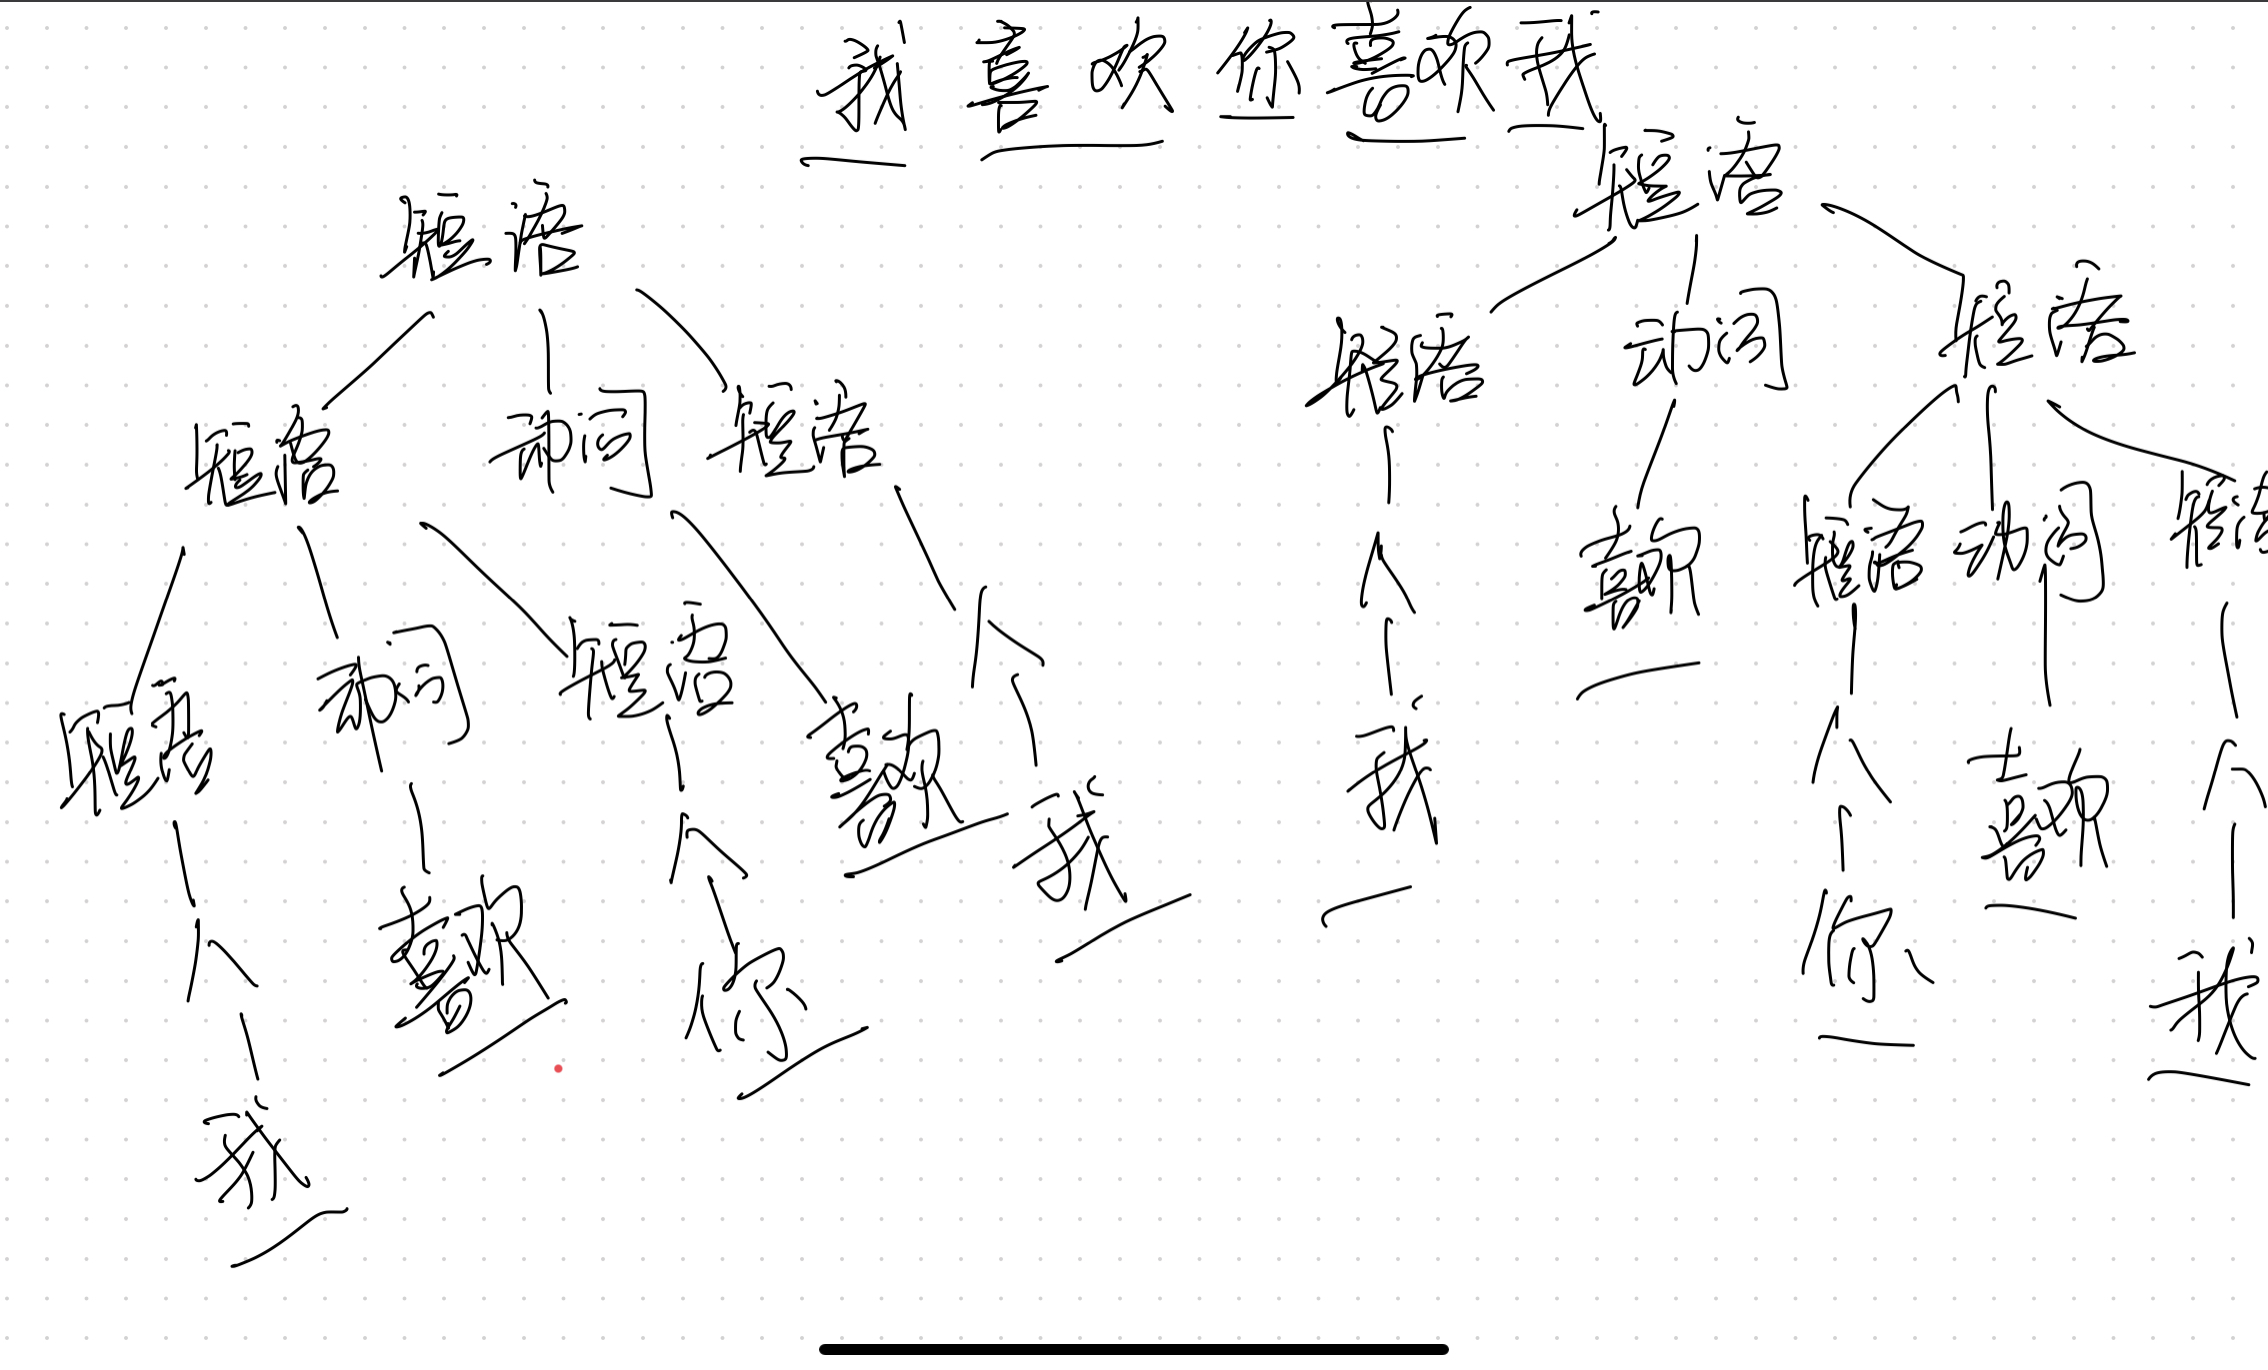
\includegraphics[width=0.9\textwidth]{img/like.jpeg}
        \caption{I like U like I}
    \end{figure}

\end{document}